Several test facilities at the Max-Planck-Institut f\"ur Physik, Munich, were developed for research and development of segmented $n$-type germanium detectors like the ones to be used in the Phase~II of the GERDA experiment. The operation and performance of several segmented detectors in vacuum and submerged in cryogenic liquid were systematically examined; various data samples were taken to investigate the event discrimination power of segmented germanium detectors. The test facilities are briefly discussed in this chapter. The data studies and analysis based on them are described in the following chapters.

\section{Cryostats}
\label{sec:tt:cryo}

\subsection{Dewar with vacuum can}
\label{sec:tt:comc}
Canberra-France developed a test cryostat shown in Fig.~\ref{fig:tt:comcryo}. A standard liquid nitrogen dewar is complemented by a two-walled aluminum vacuum can with a combined thickness of 6~mm. The detector was placed inside the can and the coordinate system was chosen such that its center was at $z=66$~mm and $r=0$~mm. The vacuum can extended to $z=116$~mm and $r=75$~mm. A copper cooling finger was used as a thermal link between the detector and the dewar. The temperature was monitored at several locations using Pt100 resistors. Liquid nitrogen was refilled daily maintaining a temperature stability of about $\pm3$~K. A comparison of spectra taken at different temperatures within this range showed neither significant differences in the general shape of the spectra nor in the energy resolution.

\begin{figure}[tbhp] 
  \centering 
  \subfloat[Dewar with vacuum can on top]{\label{fig:tt:dpc}
    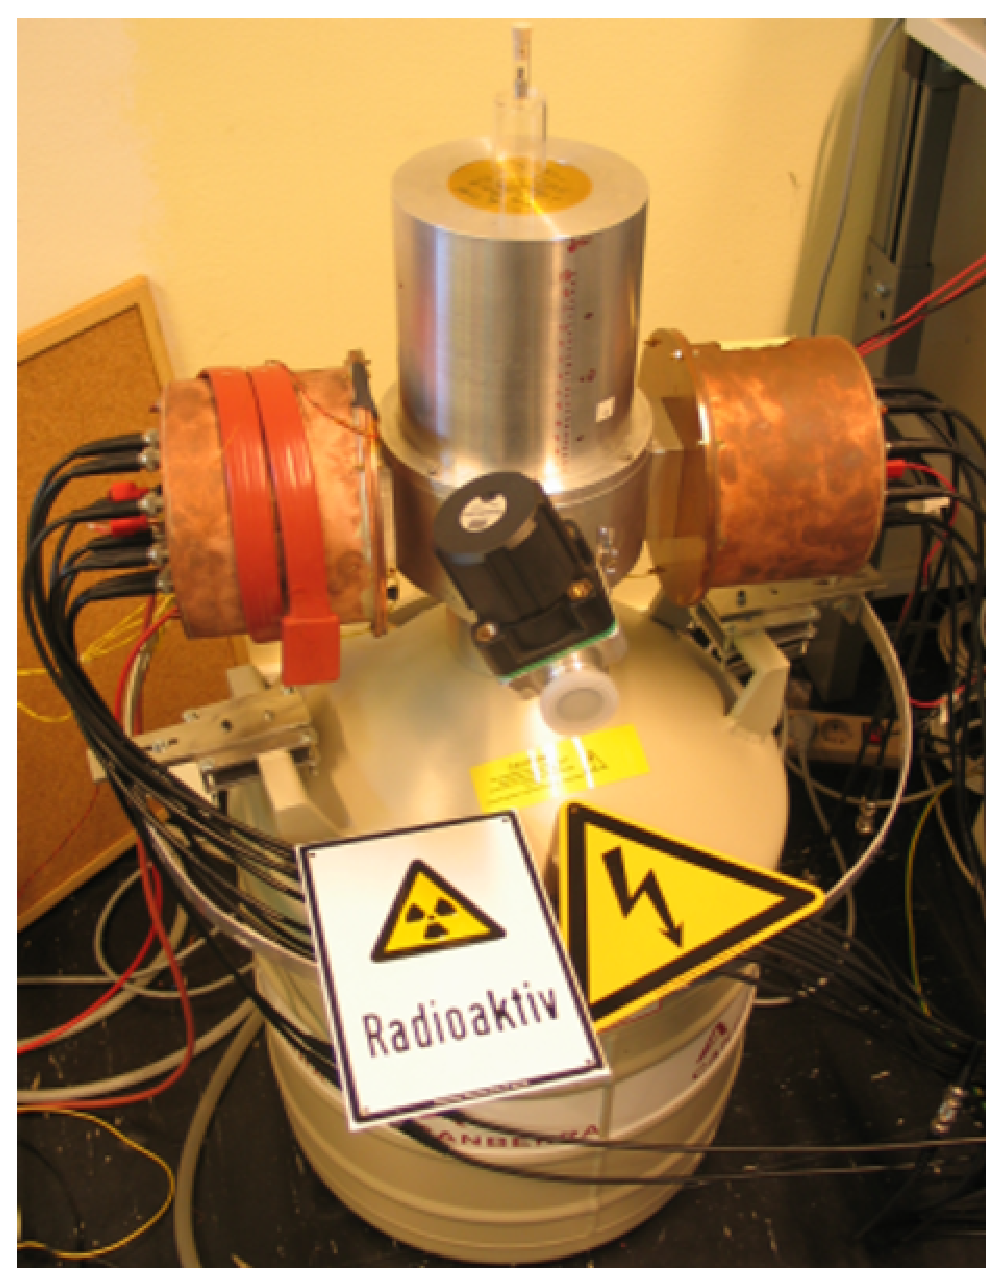
\includegraphics[height=0.25\textheight]{comcryo}}\hfil%
  \subfloat[Copper ears housing pre-amplifiers]{\label{fig:tt:ear}
    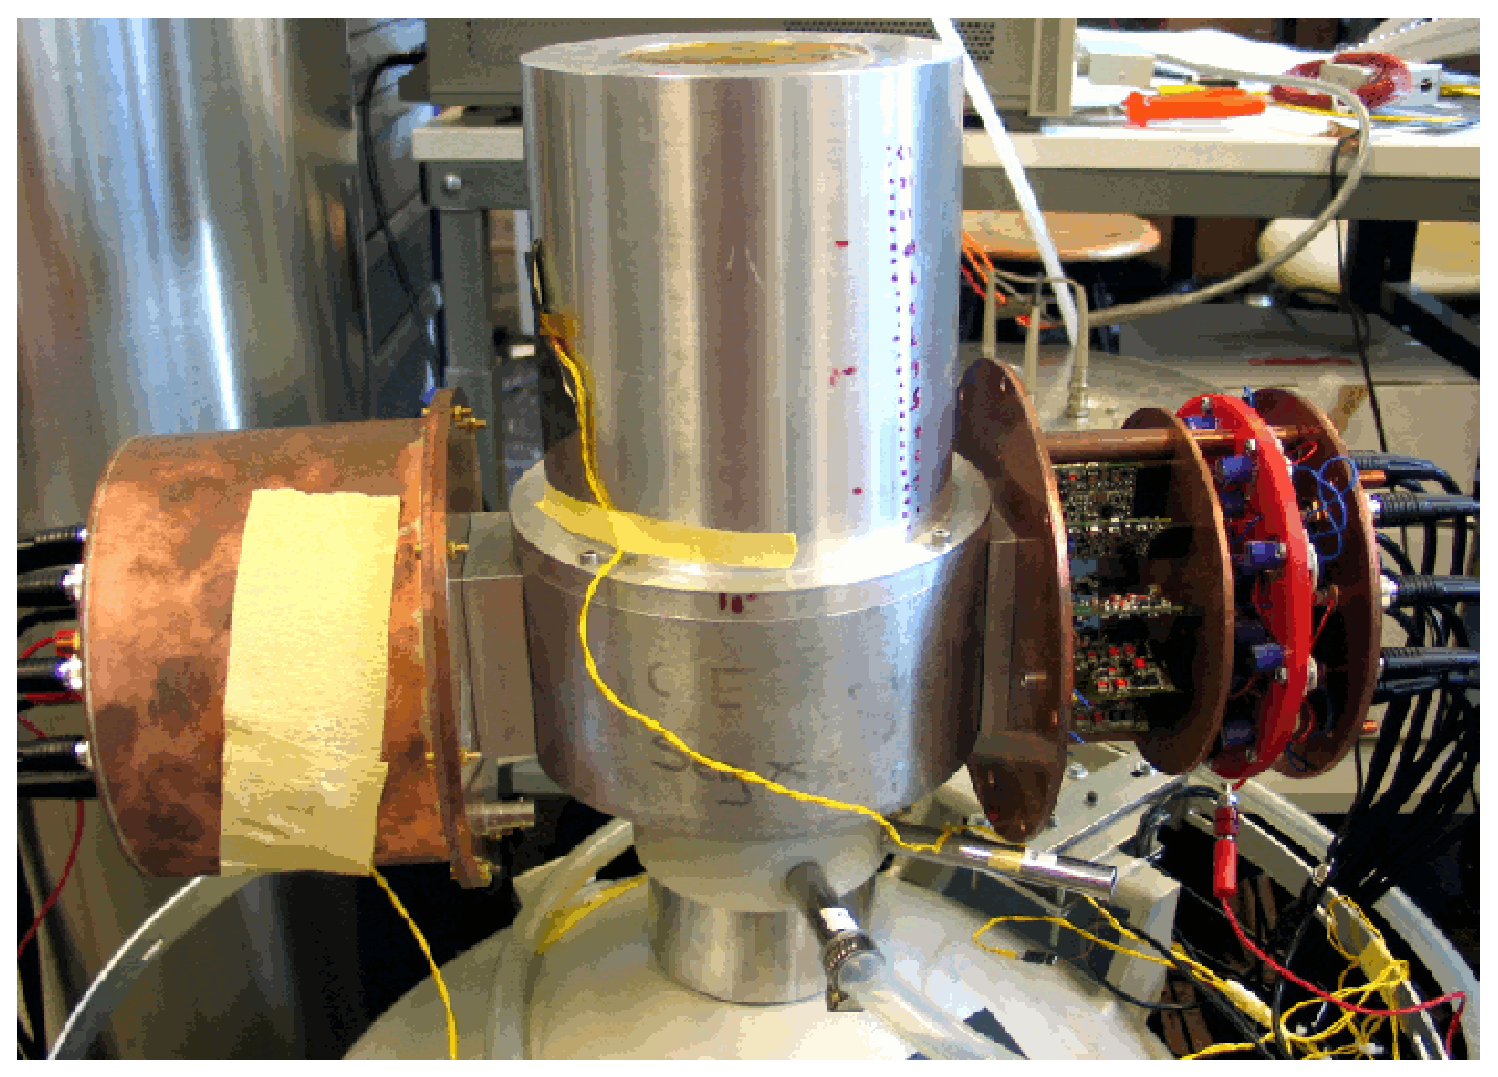
\includegraphics[height=0.25\textheight]{SIears}}%
  \caption{Test cryostat developed by Canberra-France: (a) the     standard liquid nitrogen dewar with the vacuum can on top and (b)     a close-up of the vacuum can and the copper ears housing the     pre-amplifier boards.}
  \label{fig:tt:comcryo}
\end{figure}

\subsection{Gerdalinchen II}
\label{sec:tt:gii}
Gerdalinchen II (GII in short) is a special cryostat developed by the technical division of Max-Planck-Institut f\"ur Physik to test the operation of up to three segmented germanium detectors submerged in cryogenic liquid. Fig.~\ref{fig:tt:g2} is a schematic of the main body of GII, a two-walled cryogenic dewar inside a cylindrical aluminum tank with a height of 960~mm and a diameter of 612~mm. The top flange can be removed upwards allowing the mounting of detectors to a vertical stainless steel bar under the flange, see Fig.~\ref{fig:tt:g2d}. Figure~\ref{fig:tt:g2n} shows the operation of a detector inside GII with a neutron source placed aside. 

\begin{figure}[tbhp]
  \centering
  \subfloat[Schematic of GII]{\label{fig:tt:g2}
    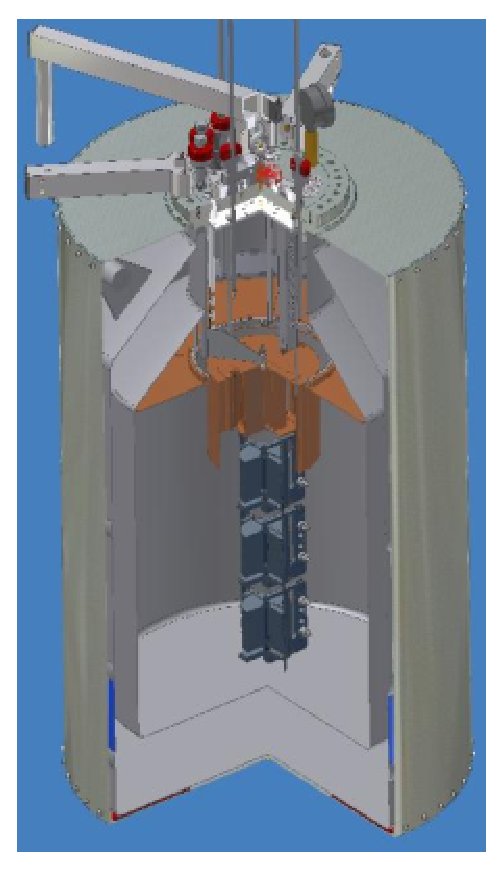
\includegraphics[height=0.25\textheight]{GIIdraw}}\hfil%
  \subfloat[GII in operation with a neutron source]{\label{fig:tt:g2n}
    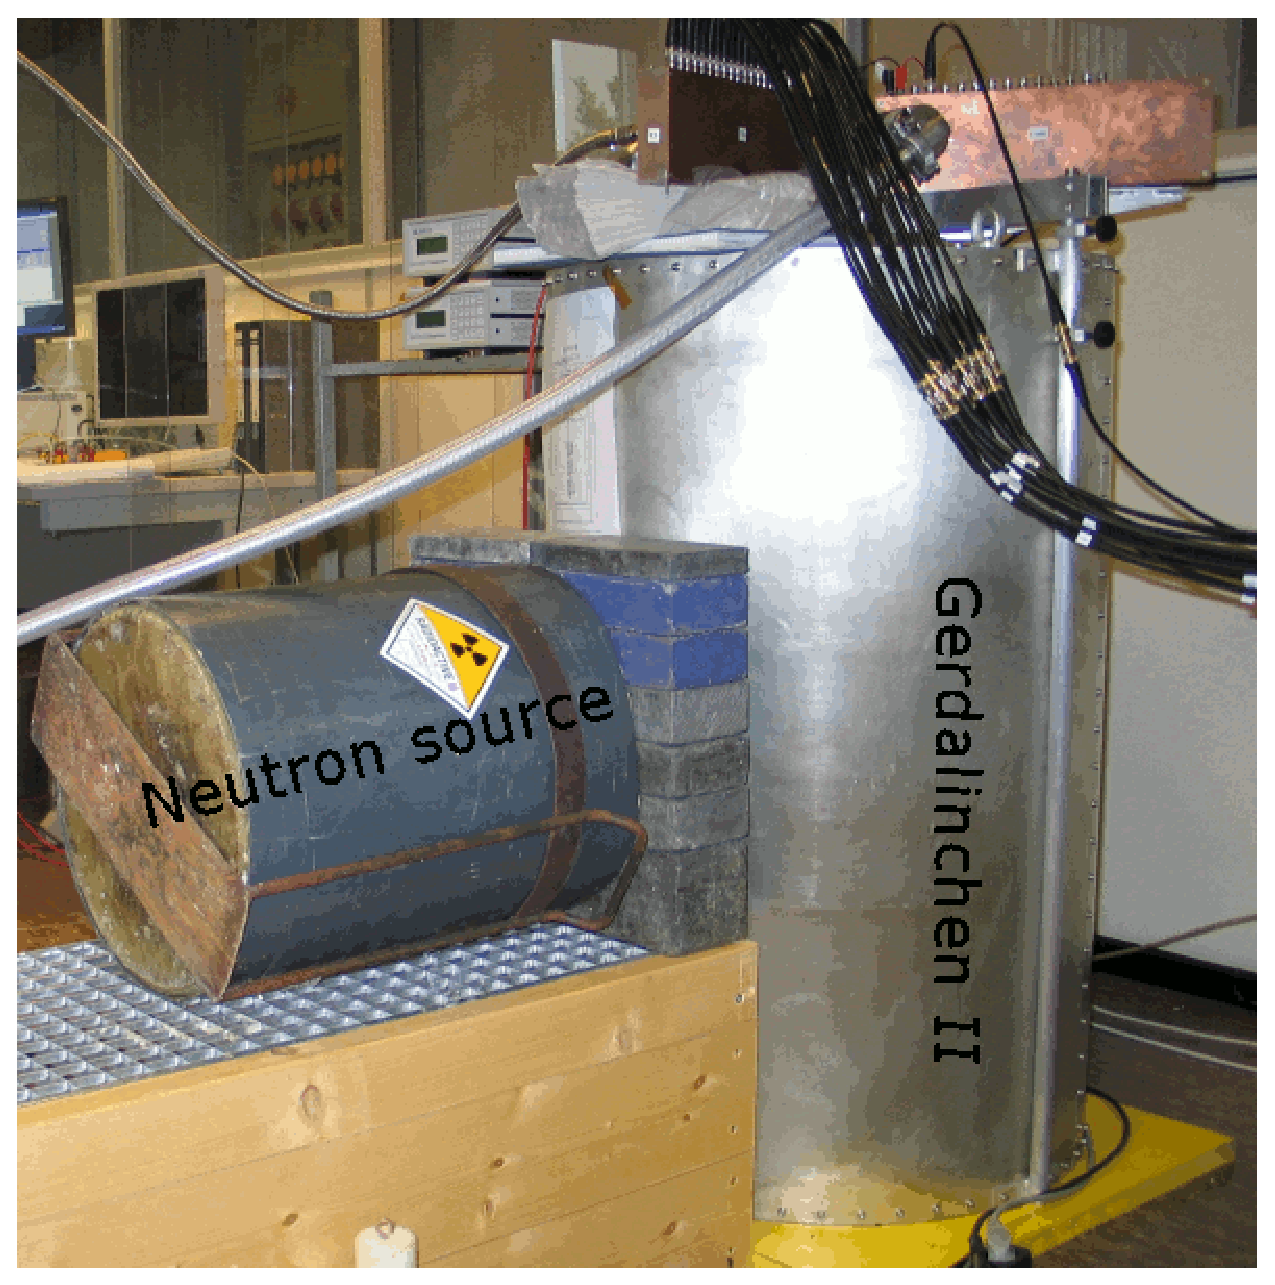
\includegraphics[height=0.25\textheight]{GIIneutron}}\hfil%
  \subfloat[Detector installation above GII dewar]{\label{fig:tt:g2d}
    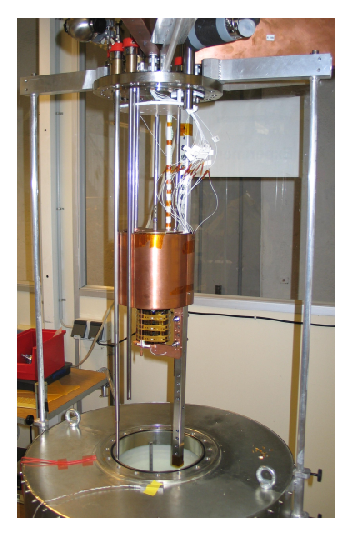
\includegraphics[height=0.25\textheight]{GIIdet}}%
  \caption{Gerdalinchen II cryostat.}
  \label{fig:tt:gii}
\end{figure}

There are three high voltage feed-throughs and four signal connectors, each with 18 channels, on the top flange. This allows the operation of three 18-fold segmented detectors simultaneously. The flange also facilitates the re-filling of the dewar with cryogenic liquid, the flushing with gaseous nitrogen and the evaluation of the dewar without opening the system. The dewar is re-filled daily to keep the level of cryogenic liquid above the infrared shields (see Fig.~\ref{fig:tt:g2}). The liquid level is monitored using several PT100 thermal resistances mounted at different places inside the dewar.


\section{Electronics} 
\label{sec:tt:ele} 

\subsection{Front-end}
\label{sec:tt:fend} 
An electronic diagram of a segmented detector mounted in the vacuum can and its read out scheme are shown in Fig.~\ref{fig:tt:sifa}. The signals were read out using charge sensitive PSC-823C pre-amplifiers[] with a decay time of 50~$\mu$s. The FET for the core electrode was mounted inside the cryostat close to the detector, the FETs for the segment electrodes were incorporated into the pre-amplifier boards which were housed inside the copper ears on both sides of the detector as shown in Fig.~\ref{fig:tt:ear}. Figure~\ref{fig:tt:sifb} depicts the layout of the feed-throughs between the vacuum can and the copper ears.

\begin{figure}[tbhp]
  \centering
  \subfloat[Read-out scheme of segmented detector mounted in the   vacuum can]{\label{fig:tt:sifa}
  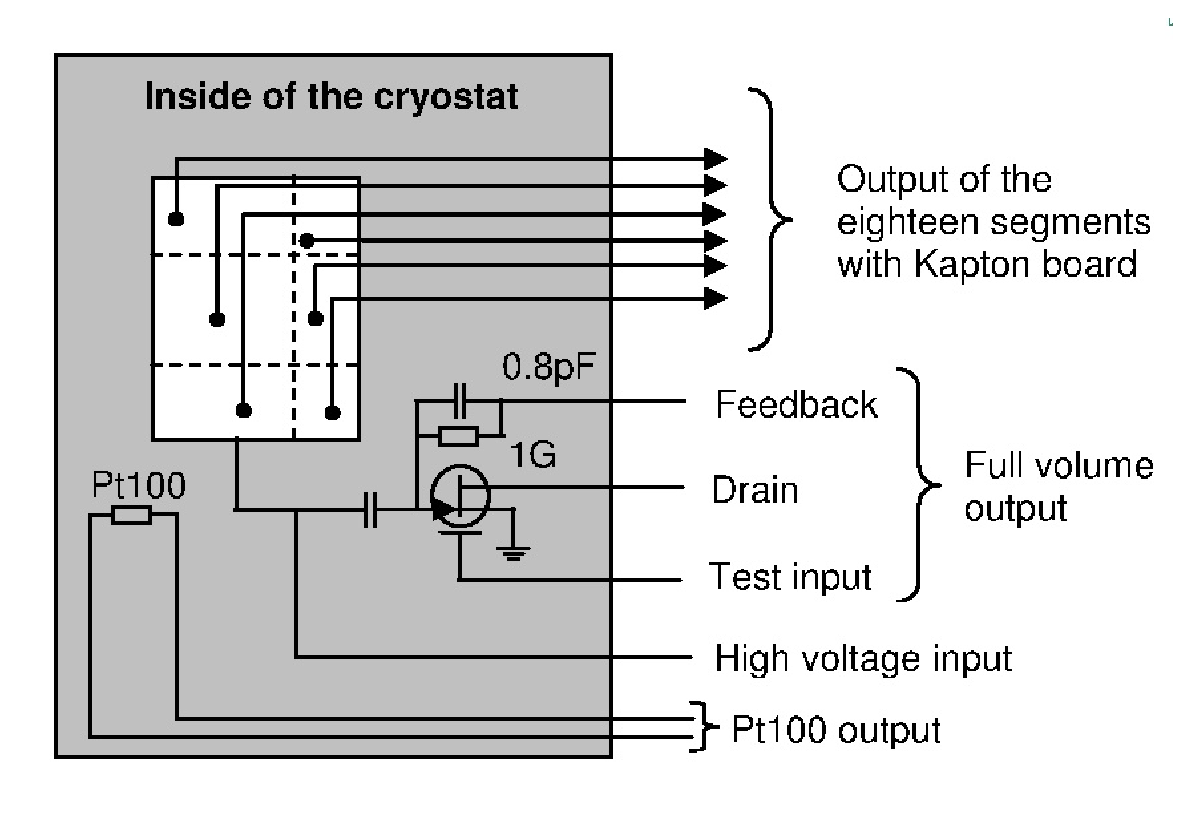
\includegraphics[height=0.25\textheight]{block1}}\hfil%
\subfloat[Layout of the feed-throughs between the vacuum can and the copper ears]{\label{fig:tt:sifb}
  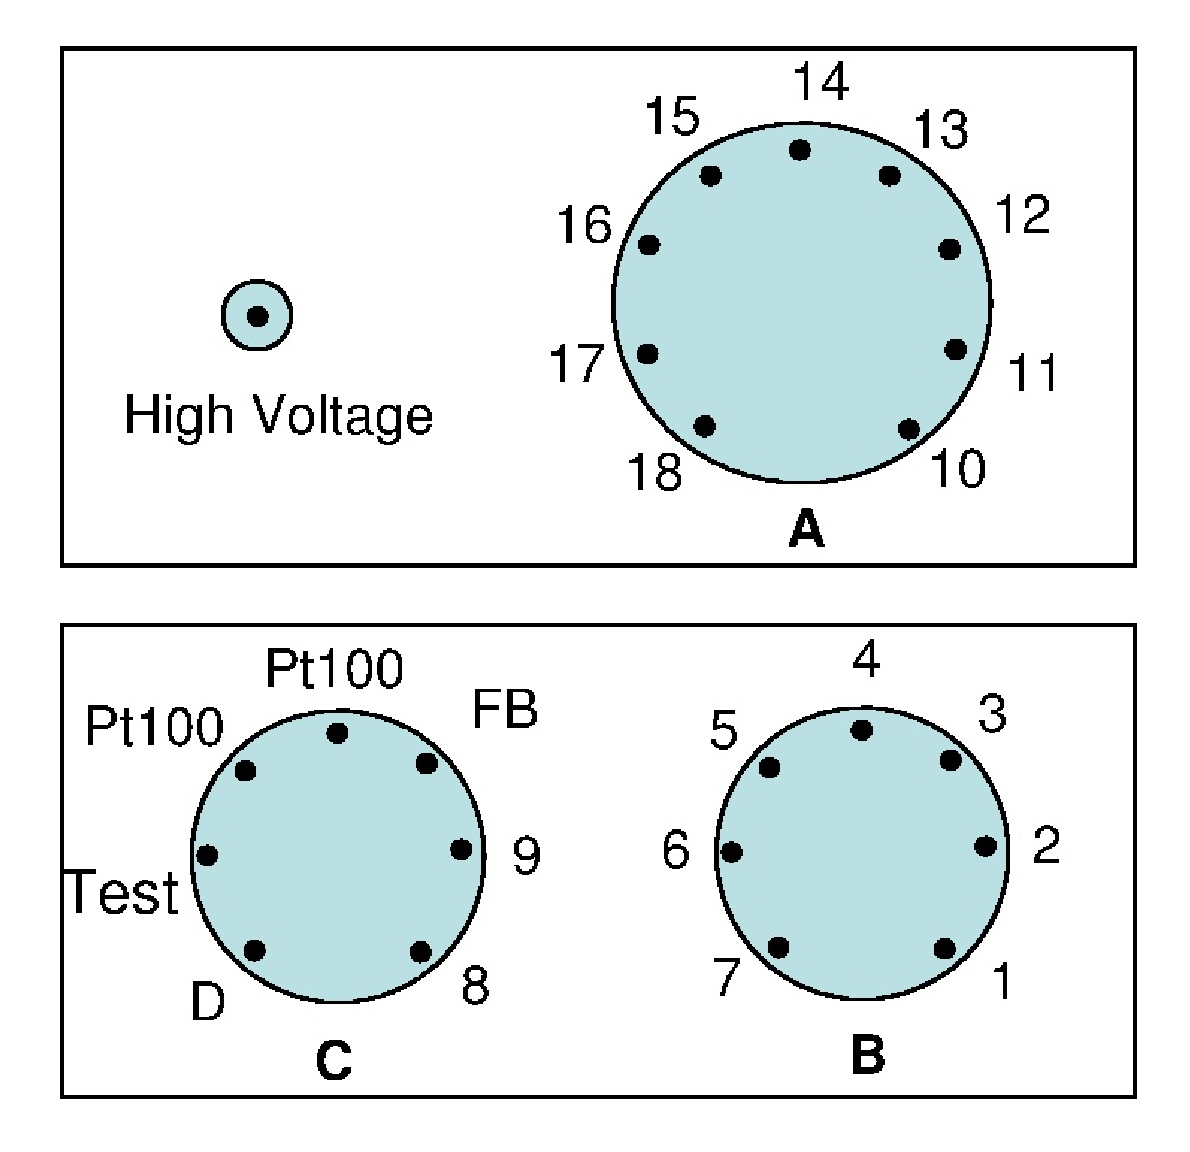
\includegraphics[height=0.25\textheight]{block2}}%
\caption{Frond-end electronics of a segmented detector mounted in the   vacuum can.}
  \label{fig:tt:sif}
\end{figure}

In GII a different setup was used. The FET for the core electrode was incorporated into the pre-amplifier boards like the segment electrodes. Thus, the cross talks from the core signal to the segment signals was minimized. All the pre-amplifier boards were mounted in a copper box and shared a common ground as shown in Fig.~\ref{fig:tt:gefb}. The filters for the high voltage lines and the coupling capacitors for the core signal cables were placed under the top flange as shown in Fig.~\ref{fig:tt:gefa}. They were first operated above the cryogenic liquid level and later submerged for better temperature stability.
\begin{figure}[tbhp]
  \centering
  \subfloat[High voltage filters and coupling capacitors in GII]{\label{fig:tt:gefa}
    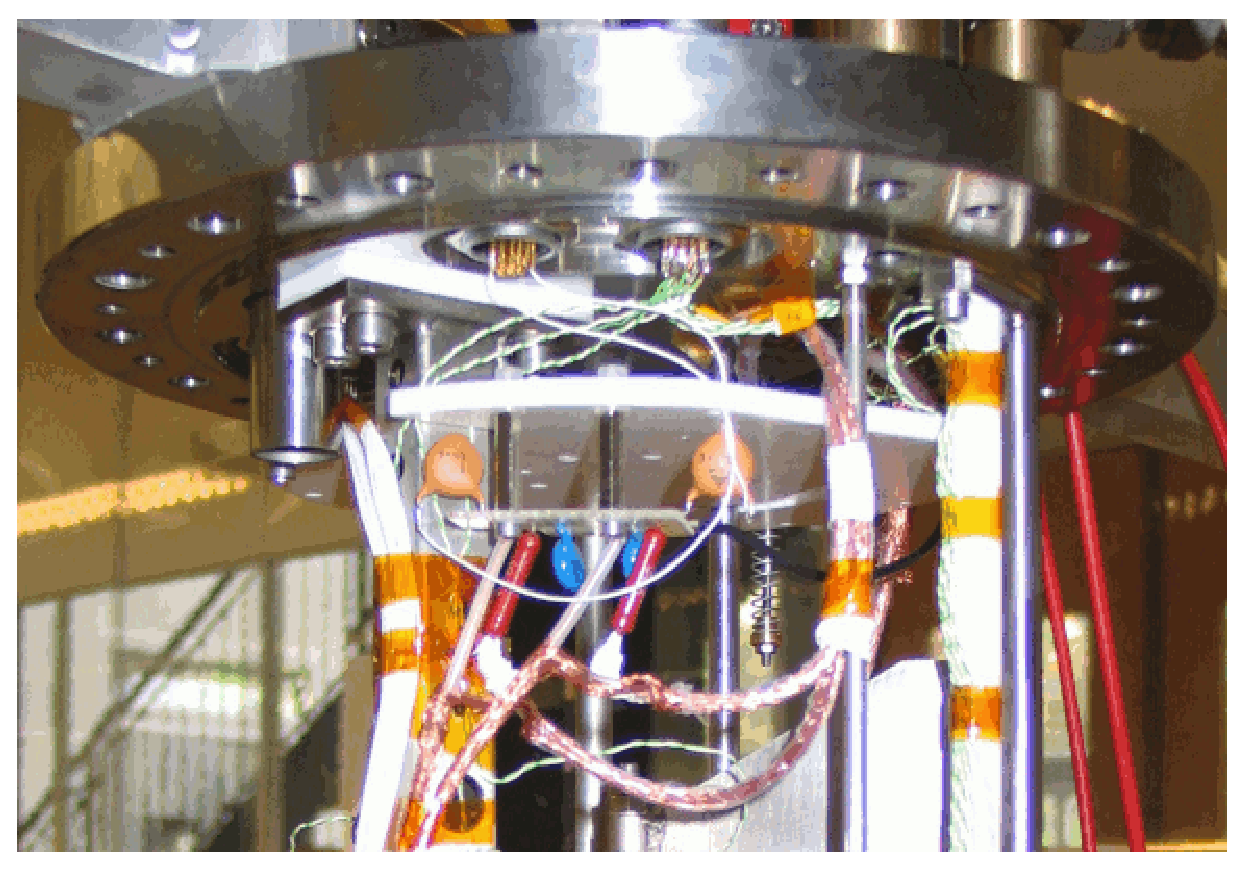
\includegraphics[height=0.2\textheight]{GIIHV}}\hfil%
  \subfloat[Pre-amplifier box for a segmented detector in GII]{\label{fig:tt:gefb}
  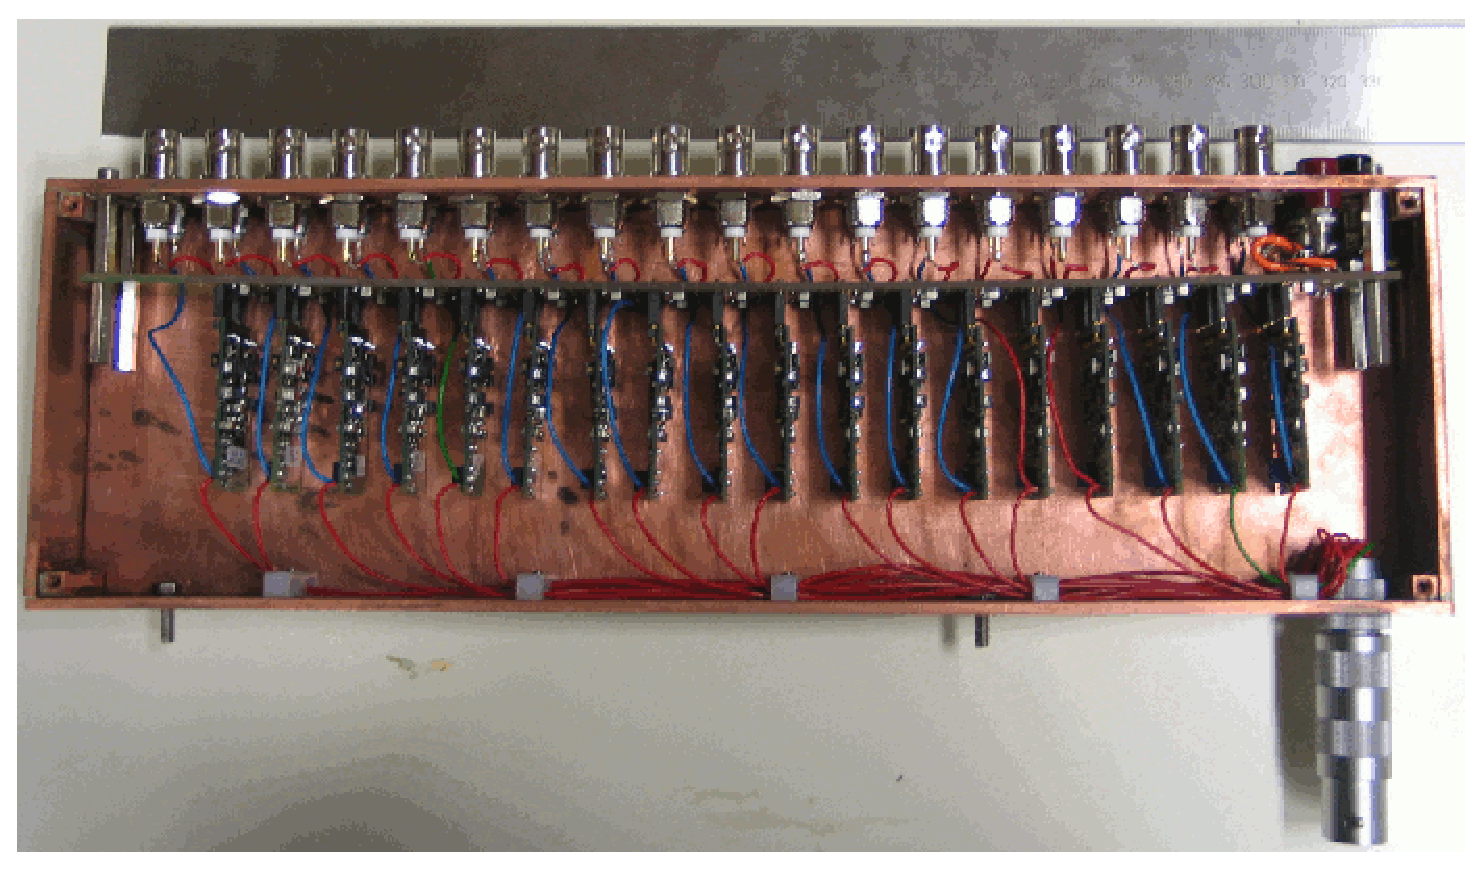
\includegraphics[height=0.2\textheight]{GIIpreamp}}%
  \caption{Front-end electronics in GII.}
  \label{fig:tt:gef}
\end{figure}

\subsection{DAQ} 
\label{sec:tt:daq}
The pre-amplified signals are digitized using an XIA data acquisition system based on 14-bit ADC PIXIE-4 modules[] with a sampling rate of 75~MHz. The bandwidth of the analog signals is limited by a Nyquist filter to half the sampling rate, \textit{i.e.} 37.5~MHz. This avoids aliasing the noise from higher frequencies. It is implemented in the analog section of the PIXIE-4 module as a low-pass Sallen-Key filter that makes a sharp (but finite) cut-off at this frequency. Energies are calculated using software filters~\cite{Pixie4}. Recorded pulse shape data consist of 300 samples of the integrated charge amplitude. The onset of the signal can be set by hand and was set to 1~$\mu$s for most of the measurements. The trigger and energy thresholds of the core and segment electrodes can be set to different values. Pile-up pulses can be rejected or stored using a rough energy estimation.


\section{Monitoring} 
\label{sec:tt:lamo}
The operation of the test facilities requires the monitoring of high voltage supplies, temperature monitors, vacuum gauges, oxygen sensors, etc. The monitoring needs to be automated for overnight or long term measurements. A generalized ``Laboratory Monitor system'', LaMo, was developed to monitor and control most of the hardware in the laboratories using the graphic programming language, LabVIEW[]. The system has a set of user friendly interfaces to perform most of the common lab tasks and a modularized design of the functionalities to facilitate the implementation of new pieces of hardware.

Fig.~\ref{fig:tt:lamo} shows the control panels of LaMo. The main panel is called ``Laboratory'' as shown in Fig.~\ref{fig:tt:plab}. It shows a list of experiments going on in the laboratory and their status. An experiment can be created, edited, started, stopped using the buttons next to the experiment list. The ``Laboratory'' panel also provides functions common to all experiments, such as email alerts, electricity, oxygen sensors, etc. Pieces of hardware to be associated to an experiment can be chosen from a list of available hardware. This is done in the ``Config'' panel of LaMo as shown in Fig.~\ref{fig:tt:pcon}, where pieces of hardware can be added, deleted from the list to be monitored. Once an experiment is created and configured, it is started from the ``Laboratory'' panel. An ``Experiment'' panel, as shown in Fig.~\ref{fig:tt:pexp}, where monitored variables are shown in different ways, automatically pop up. The functions specified for a particular experiment can be executed from there.

\begin{figure}[tbhp]
  \centering
  \subfloat[``Laboratory'' panel]{\label{fig:tt:plab}
    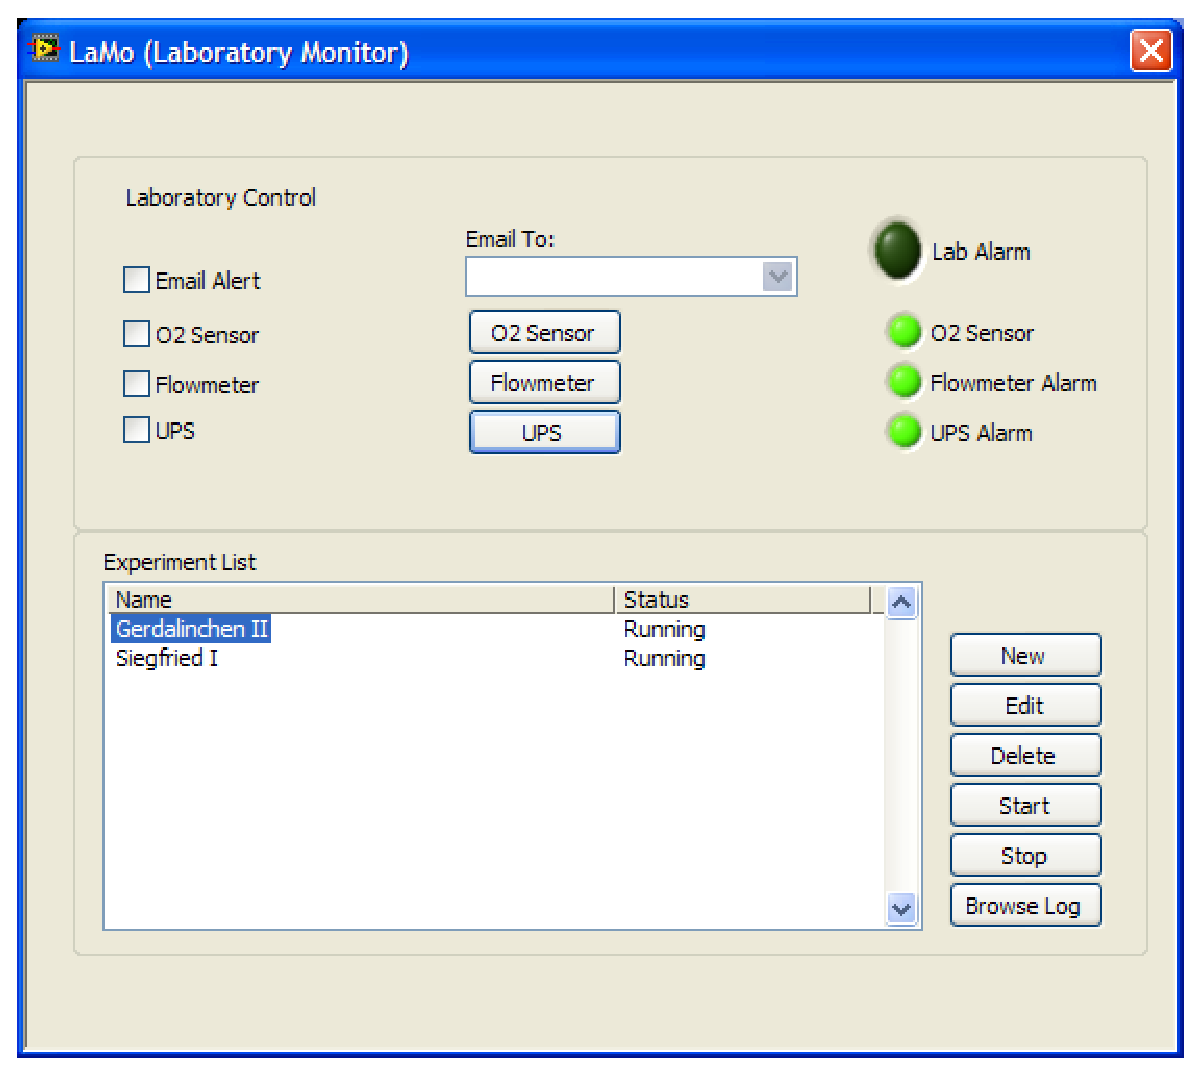
\includegraphics[height=0.23\textheight]{LaMoLab}}\hfil%
  \subfloat[``Config'' panel]{\label{fig:tt:pcon}
  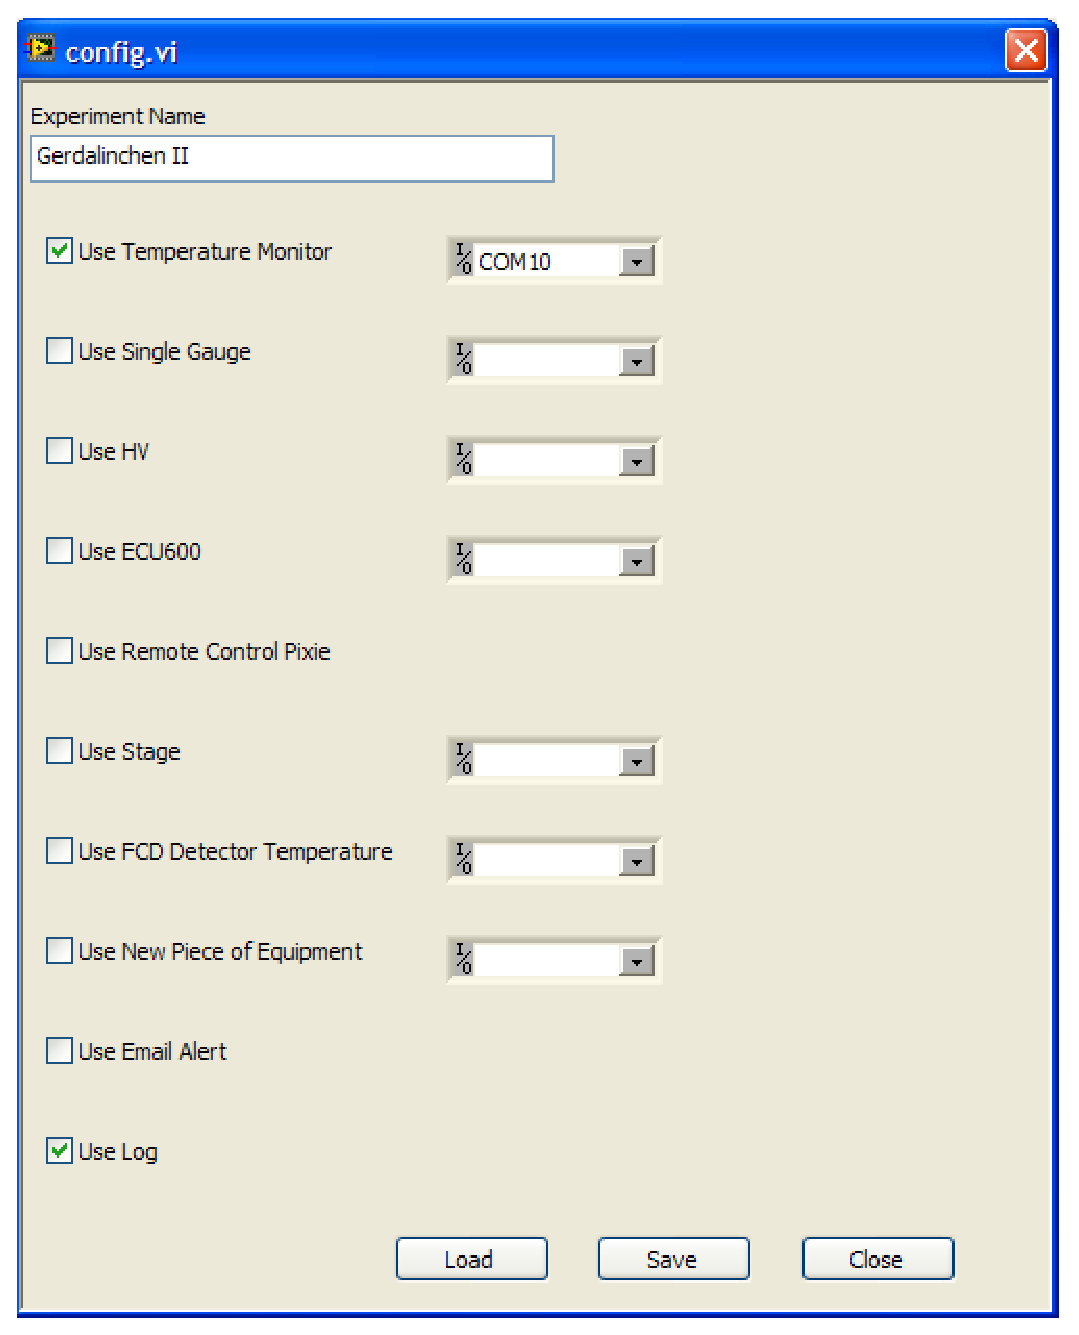
\includegraphics[height=0.23\textheight]{LaMoEdit}}\hfil%
  \subfloat[``Experiment'' panel]{\label{fig:tt:pexp}
  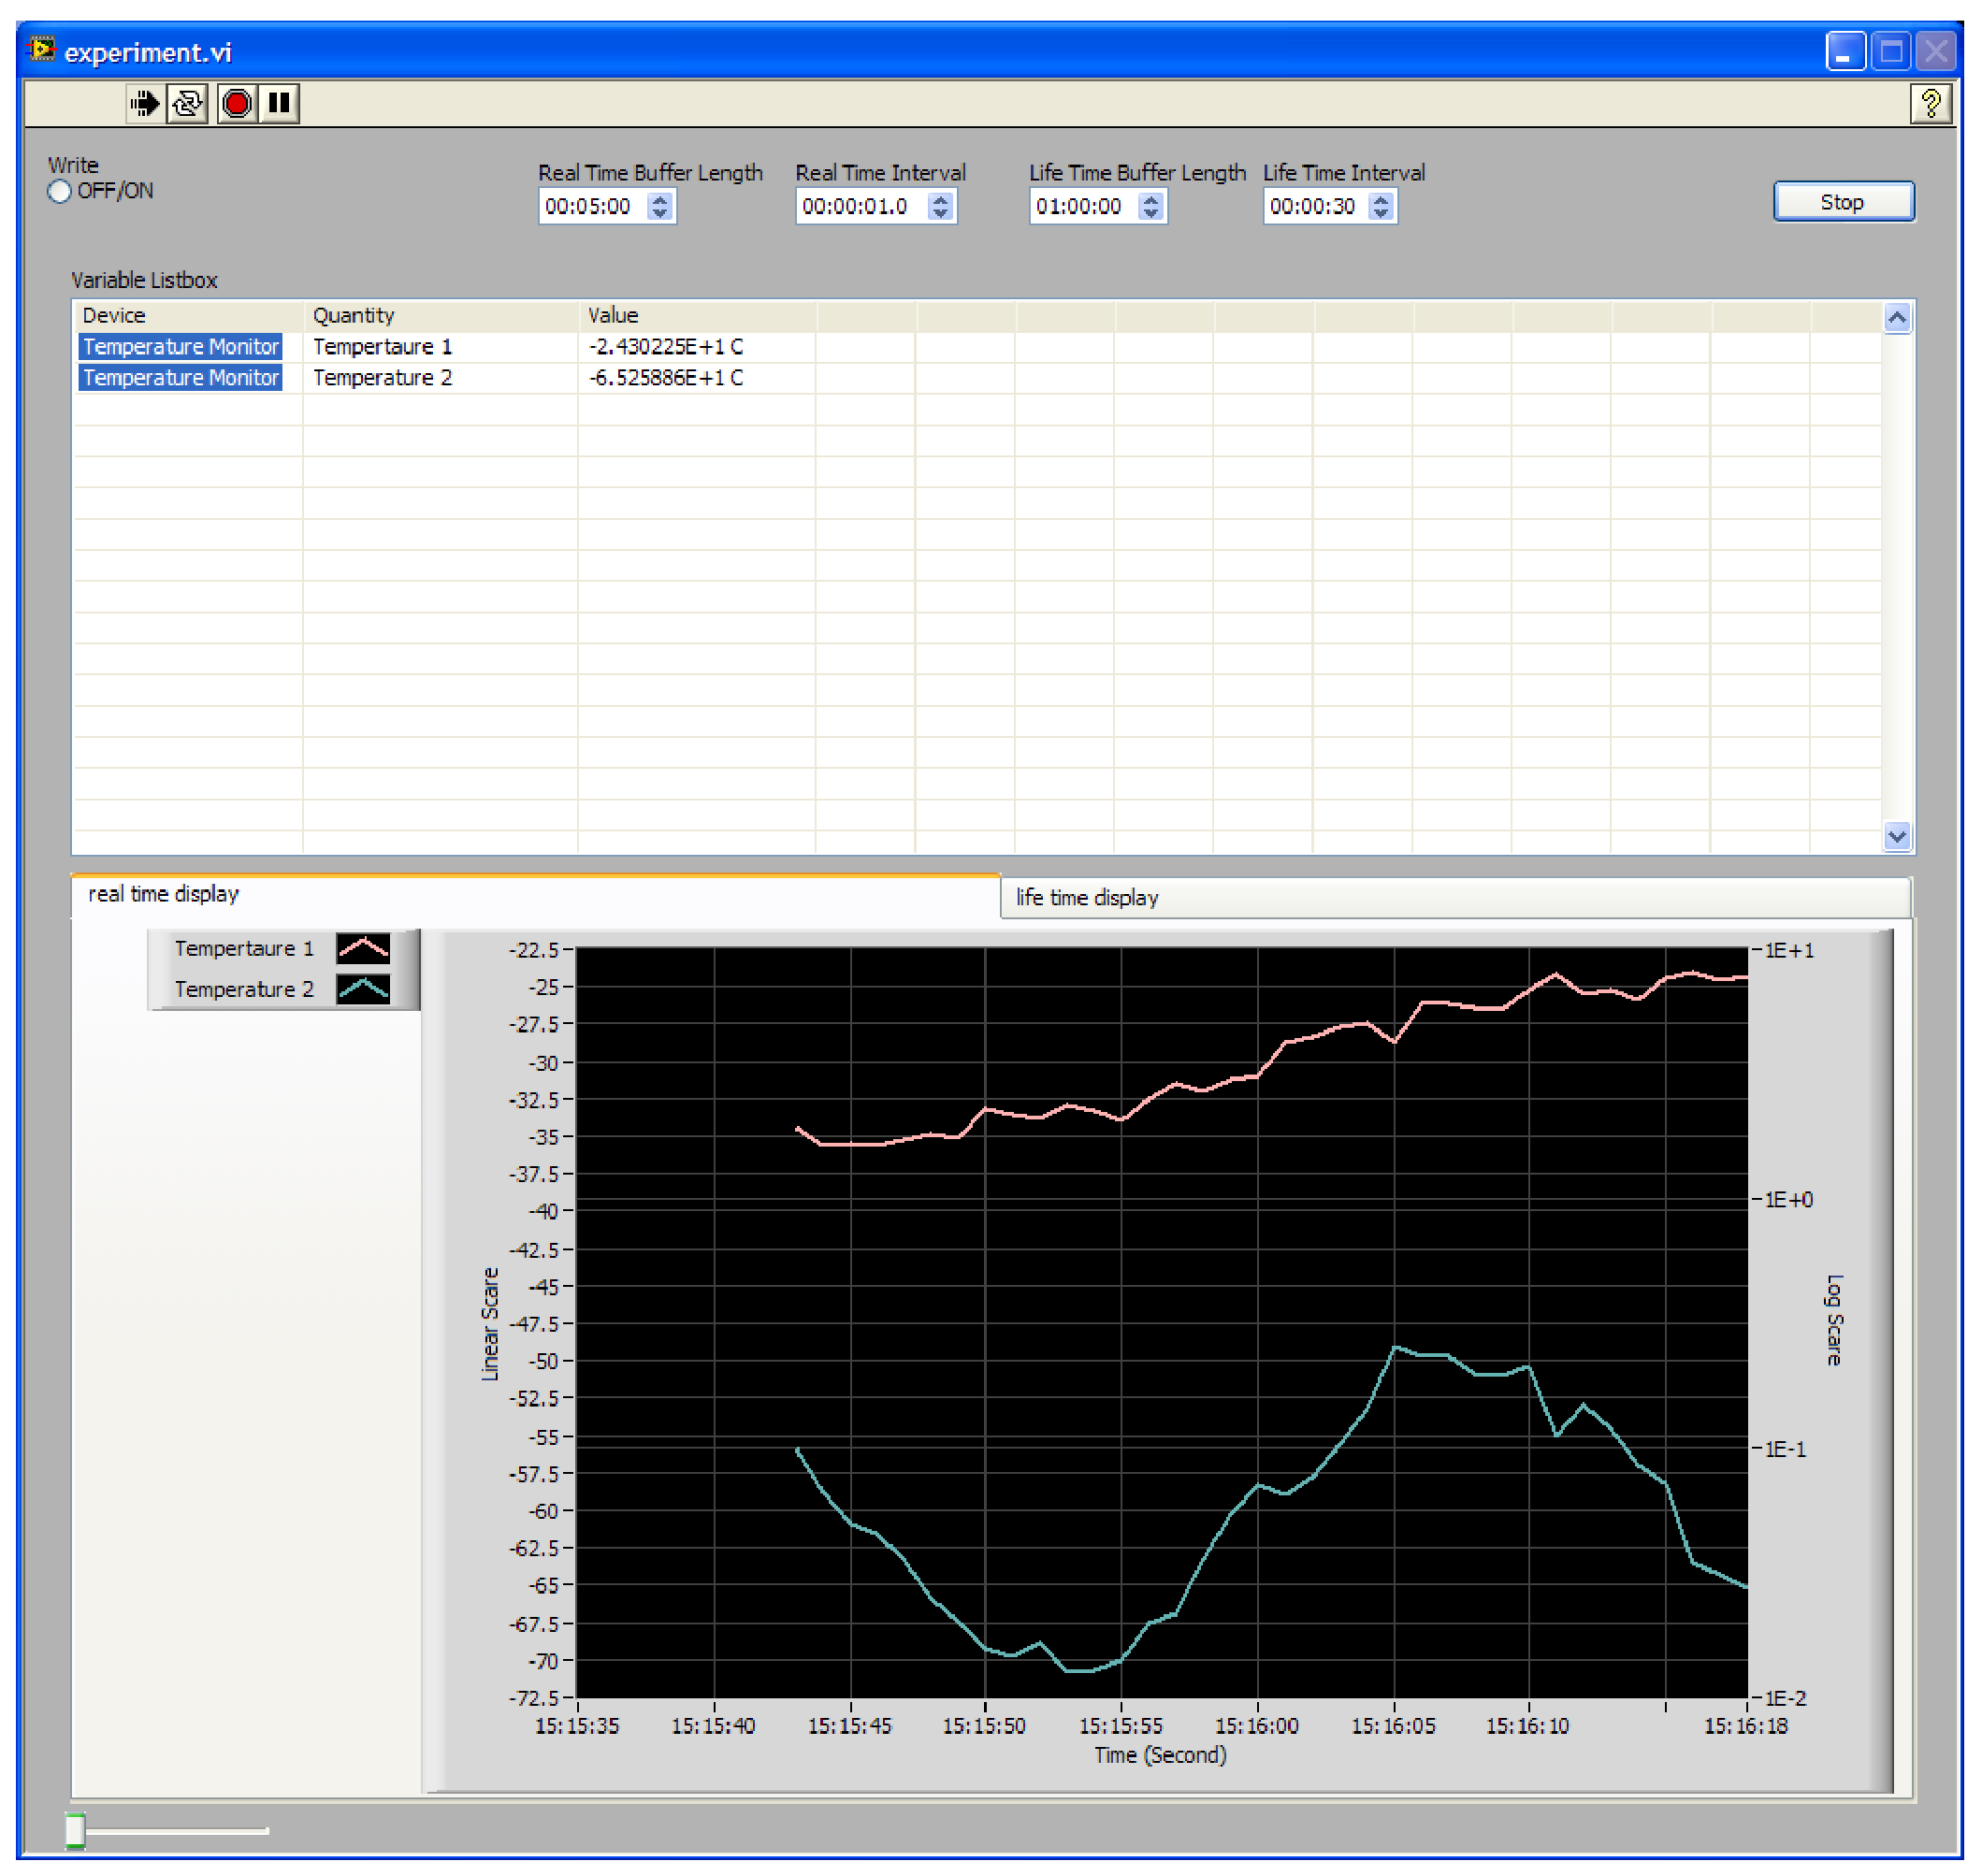
\includegraphics[height=0.23\textheight]{LaMoExp}}%
  \caption{Main panels of LaMo: (a) ``Laboratory'' panel: it provides a list of experiments and their status, and gives access to functions common to all experiments; (b) ``Config'' panel: pieces of hardware to be associated to an experiment can be added, deleted from the list to be monitored; (c) ``Experiment'' panel: various displays of monitored variables can be requested and the execution of experimental tasks can be steered.}
  \label{fig:tt:lamo}
\end{figure}

The common user interface enforces common I/Os for different pieces of hardware. The functionality of LaMo is modularized so that the effort to implement a new piece of hardware is minimized. To add a new piece of equipment the developer only needs to define its I/O interface to LaMo. The other efforts, such as programming the user interface, etc., do not have to be repeated every time.


%%% Local Variables:
%%% mode:latex
%%% TeX-master: "thesis"
%%% End:
